\subsection{Διασύνδεση υπηρεσιών} \label{subsection:4-3-8-service-communication}

Βασικό χαρακτηριστικό του μοντέλου των μικροϋπηρεσιών είναι η επικοινωνία των ξεχωριστών υπηρεσιών και η ανταλλαγή μηνυμάτων για την επίτευξη των λειτουργιών του συστήματος. Σε αυτήν την υποενότητα θα αναλυθεί ο τρόπος με τον οποίον οι μικροϋπηρεσίες επικοινωνούν μεταξύ τους, καθώς και η φύση και το περιεχόμενο των μηνυμάτων που ανταλλάσουν.

Στο παρακάτω σχήμα (σχήμα \ref{figure:4-3-communications-graph}) φαίνεται ο γράφος που οπτικοποιεί τα κανάλια επικοινωνίας μεταξύ των μικροϋπηρεσιών, καθώς και τα κανάλια επικοινωνίας των μικροϋπηρεσιών με το blockchain.

\begin{figure}[H]
    \centering
    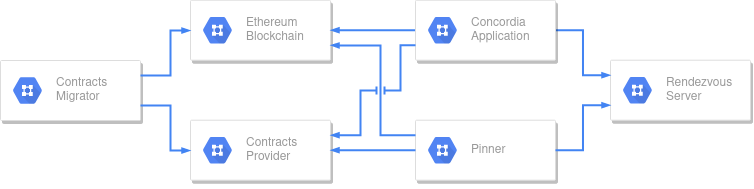
\includegraphics[width=\textwidth]{assets/figures/chapter-4/4.3.communications-diagram}
    \caption{Γράφος οπτικοποίησης των καναλιών επικοινωνίας των μικροϋπηρεσιών}
    \label{figure:4-3-communications-graph}
\end{figure}

Εδώ αναλύεται η επικοινωνία κάθε μικροϋπηρεσίας:

\begin{itemize}
    \item \textbf{Contracts Migrator}: Η υπηρεσία εκτελεί αίτημα HTTP κατά τη μεταφόρτωση των \textenglish{contract} στο Ethereum blockchain. Eπίσης, εκτελεί αίτημα HTTP για τη μεταφόρτωση των \textenglish{contract artifact} στην υπηρεσία Contracts Provider.

    \item \textbf{Concordia Application}: Η υπηρεσία εκτελεί αίτημα HTTP για τη λήψη των \textenglish{contract artifact} από την υπηρεσία Contracts Provider, εκτελεί αιτήματα HTTP για τη διενέργεια συναλλαγών στο Ethereum blockchain και, τέλος, δημιουργεί κανάλι επικοινωνίας UDP με την υπηρεσία Rendezvous Server, για την ανακάλυψη ομότιμων χρηστών στο δίκτυο IPFS.

    \item \textbf{Pinner}: Η υπηρεσία εκτελεί αίτημα HTTP για τη λήψη των \textenglish{contract artifact} από την υπηρεσία Contracts Provider, εκτελεί αιτήματα HTTP για την ανανέωση και παρατήρηση της κατάστασης του contract στο Ethereum blockchain και τέλος δημιουργεί κανάλι επικοινωνίας UDP με την υπηρεσία Rendezvous Server για την ανακάλυψη peer στο δίκτυο IPFS.

    \item \textbf{Rendezvous Server}: Η υπηρεσία διατηρεί ανοιχτά κανάλια επικοινωνίας UDP με τους ομότιμους χρήστες, μέσω των οποίων ενημερώνει τη λίστα των διαθέσιμων, ενεργών χρηστών.

    \item \textbf{Contracts Provider}: Η υπηρεσία δεν υποκινεί καμία επικοινωνία, παρά μόνο απαντά σε αιτήματα επικοινωνίας από άλλες υπηρεσίες.
\end{itemize}